\documentclass{article}%
\usepackage[T1]{fontenc}%
\usepackage[utf8]{inputenc}%
\usepackage{lmodern}%
\usepackage{textcomp}%
\usepackage{lastpage}%
\usepackage[head=40pt,margin=0.5in,bottom=0.6in]{geometry}%
\usepackage{graphicx}%
%
\title{\textbf{El Aissami: medidas de EEUU impiden adquirir medicinas}}%
\author{MAGALY PEREZ}%
\date{10/10/2018}%
%
\begin{document}%
\normalsize%
\maketitle%
\textbf{URL: }%
http://www.eluniversal.com/economia/22781/el{-}aissami{-}medidas{-}de{-}eeuu{-}impiden{-}adquirir{-}medicinas\newline%
%
\textbf{Periodico: }%
EU, %
ID: %
22781, %
Seccion: %
economia\newline%
%
\textbf{Palabras Claves: }%
NO\_TIENE\newline%
%
\textbf{Derecho: }%
2.1, %
Otros Derechos: %
, %
Sub Derechos: %
2.1.1\newline%
%
\textbf{EP: }%
NO\newline%
\newline%
%
\textbf{\textit{Cree que la ONU debe obligar a USA a levantar sanciones contra Venezuela}}%
\newline%
\newline%
%
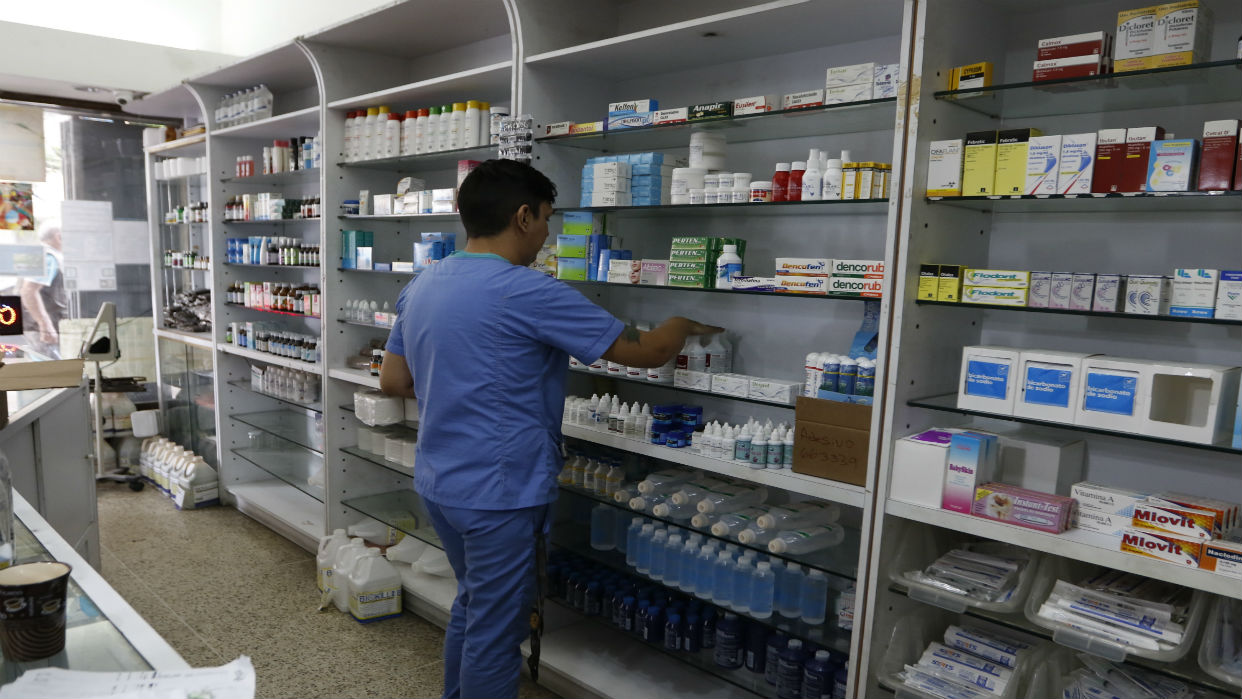
\includegraphics[width=300px]{205.jpg}%
\newline%
%
Caracas.{-}Las sanciones impuestas a Venezuela por Estados Unidos impiden que el gobierno venezolano tenga la posibilidad de adquirir medicamentos, y otros insumos y bienes necesarios para el desarrollo de cualquier país.%
\newline%
%
Así lo afirmó el vicepresidente sectorial del Área Económica, Tareck El Aissami, durante una entrevista concedida al medio de comunicación ruso RT.%
\newline%
%
El funcionario aseveró que las sanciones aplicadas contra nuestro país “son ilegales, arbitrarias y violatorias del derecho internacional, pero por otro lado, sostienen un discurso manipulador de una supuesta ayuda humanitaria”.%
\newline%
%
En ese sentido, el Vicepresidente Sectorial puntualizó que la mejor ayuda sería levantar las sanciones, e instó a las “Naciones Unidas a que saque una resolución contra Estados Unidos para que levante este tipo de abusos y arbitrariedades que violan el derecho internacional”.%
\newline%
%
En cuanto a la espera de los precios acordados de los medicamentos que aún están en análisis, Freddy Cevallos presidente de la Federación Farmacéutica de Venezuela (Fefarven), señaló que la aplicación de estos precios no será la solución a la crisis de fármacos.%
\newline%
%
Indicó que por parte del Estado se ha planteado el subsidio y que la vigencia de los costos tenga un lapso de tres meses.%
\newline%
%
Sin embargo, Cevallos insiste en que “hay que estimular la producción de medicamentos, para que el país empiece a funcionar”, expresó, el presidente de Fefarven.%
\newline%
%
El dirigente señaló que aún los resultados de estas reuniones están en consideración.%
\newline%
%
Agregó que se ha tomado como prioridad los medicamentos esenciales; los que cubran la mayoría de las patologías en el país.%
\newline%
%
Pero las farmacias en el país se encuentran en estado crítico y según Cevallos, 150 farmacias han cerrado en un lapso de año y medio, producto de la crisis económica.%
\newline%
%
Por su parte, Tito López presidente de la Cámara de la Industria Farmacéutica Venezolana, señaló que en el gremio existe el temor de que los precios que se acuerden con el Ejecutivo Nacional de un grupo de medicamentos, no sean revisados constantemente.%
\newline%
%
Dijo que la Sundde debe garantizar la revisión de los precios cada dos meses.%
\newline%
%
El gremio espera por la reunión con el sector gobierno.%
\newline%
%
\end{document}